\documentclass[fleqn,usenatbib]{mnras}

\usepackage[T1]{fontenc}
\usepackage{graphicx}
\usepackage{booktabs}
\usepackage{amsmath}
\usepackage{amssymb}
\usepackage{url}

\title[Candidate-conditioned transit inference]{TransitFlow: flow-matching posterior estimation for candidate-conditioned exoplanet transit inference}

\author[Author et al.]{Author Name$^{1}$\thanks{E-mail: author@example.org}\\
$^{1}$Affiliation to be supplied before submission}

\date{Accepted XXX. Received YYY; in original form ZZZ}
\pubyear{2026}

\begin{document}
\label{firstpage}
\pagerange{\pageref{firstpage}--\pageref{lastpage}}
\maketitle

\begin{abstract}
We present TransitFlow, a candidate-conditioned simulation-based inference
pipeline that combines a transit-candidate probability with a flow-matching
posterior over $R_{\rm p}/R_\star$, $a/R_\star$, impact parameter $b$, and two
quadratic limb-darkening parameters. The method consumes global, candidate-folded
local, and box-periodogram views of TESS-like light curves. A
target-disjoint development experiment rejects marginal simulation-based
calibration for three of five parameters despite a mean absolute coverage error
of 0.015. We trace this failure to a clipped stellar-density prior and a mismatch
between bounded posterior targets and the Gaussian flow base, and introduce an
exact truncated prior with a conditional prior-CDF-to-normal transformation. A
small end-to-end smoke passes posterior calibration diagnostics but fails the
detection threshold and is not treated as scientific evidence. We also correct an
evaluation design in which the neural classifier received the simulated true
ephemeris while Box Least Squares (BLS) had to search. In a corrected
$n=1000$ candidate-vetting experiment, TransitFlow achieves ROC-AUC $0.807$
(95 per cent paired-bootstrap interval $0.782$--$0.834$) and average precision
$0.762$ ($0.731$--$0.796$), compared with $0.598$ and $0.584$ for the BLS score.
This pilot predates the frozen target-level protocol. A selected positive-only
sample recovers 30 known TESS
transits, but does not establish real-world reliability, and previous
real-posterior agreement values are invalidated by collapsed importance-sampling
effective sample size and unconverged MCMC references. TransitFlow is a
promising candidate-conditioned method, not yet a validated blind-search or
real-characterization system.
\end{abstract}

\begin{keywords}
methods: data analysis -- methods: statistical -- planets and satellites:
detection -- techniques: photometric
\end{keywords}

\section{Introduction}
\label{sec:introduction}

Transit surveys require both candidate discovery and physical interpretation.
Box Least Squares (BLS; \citealt{Kovacs2002}) and Transit Least Squares
(TLS; \citealt{Hippke2019}) provide effective periodic-search statistics,
whereas learned vetters such as AstroNet \citep{Shallue2018} and ExoMiner
\citep{Valizadegan2022} classify threshold-crossing events from richer data
products. Those systems are primarily optimized for discrimination. Physical
transit parameters and their uncertainties are normally inferred in a second
stage using likelihood-based sampling; joint Bayesian detection and noise
characterization has also been explored \\citep{Taaki2020}.

Simulation-based inference (SBI) offers a complementary route when a forward
simulator is available but repeated posterior sampling is expensive
\citep{Cranmer2020,Lueckmann2021}. Neural posterior estimators amortize the cost
of inference over simulations. Their scientific utility nevertheless depends on
calibration and fidelity rather than predictive accuracy alone; apparently
plausible neural posteriors can be unfaithful \citep{Hermans2022}, motivating
simulation-based calibration (SBC; \citealt{Talts2018}), expected-coverage
tests, posterior predictive checks and explicit out-of-distribution diagnostics.

Flow-matching posterior estimation (FMPE) applies continuous flow matching
\citep{Lipman2023} to SBI \citep{Dax2023}. It has been demonstrated for
exoplanet atmospheric retrieval \citep{Gebhard2025}. Conditional flow matching
has also been used for transit-light-curve classification \citep{Fiscale2025}.
TransitFlow therefore does not claim the first use of flow matching for transit
detection, nor a new flow-matching algorithm. Its intended contribution is
narrower: an FMPE posterior for candidate-conditioned transit photometry,
coupled to a candidate probability and evaluated with calibration and
misspecification diagnostics.

This paper has two aims. First, we define the model and the astronomical task
without conflating candidate vetting with blind search. Secondly, we audit the
available evidence under that definition. The audit uncovered privileged
ephemeris information in the original detection benchmark, a non-independent
noise evaluation, and invalid importance-resampled real-posterior comparisons.
We correct the corresponding code paths and report only the results that remain
interpretable. The resulting manuscript is deliberately a pre-submission draft:
Section~\ref{sec:blockers} states the experiments that must be completed before
the method can support an MNRAS submission.

\section{Problem formulation}
\label{sec:problem}

Let $x$ denote a single-sector light curve and $c=(P,t_0)$ a proposed candidate
ephemeris. TransitFlow models the factorization
\begin{equation}
 p(d,\boldsymbol{\theta}\mid x,c) =
 p(d\mid x,c)\,p(\boldsymbol{\theta}\mid d=1,x,c),
\end{equation}
where $d$ indicates whether the candidate is transit-like and
\begin{equation}
 \boldsymbol{\theta} =
 (R_{\rm p}/R_\star, a/R_\star, b, q_1, q_2).
\end{equation}
The period and epoch are conditioning variables rather than posterior targets.
This distinction is important: posterior plots or coverage statistics for
$P$ and $t_0$ would not measure characterization calibration in the present
five-dimensional model.

The factorization is implemented by two heads sharing an observation embedding
(Fig.~\ref{fig:architecture}). It is a practical joint interface, but not a
single mixed discrete--continuous posterior. At deployment, BLS or TLS must
propose $c$. A benchmark that supplies the true positive ephemeris measures an
oracle-candidate diagnostic, not end-to-end discovery.

\begin{figure*}
 \centering
 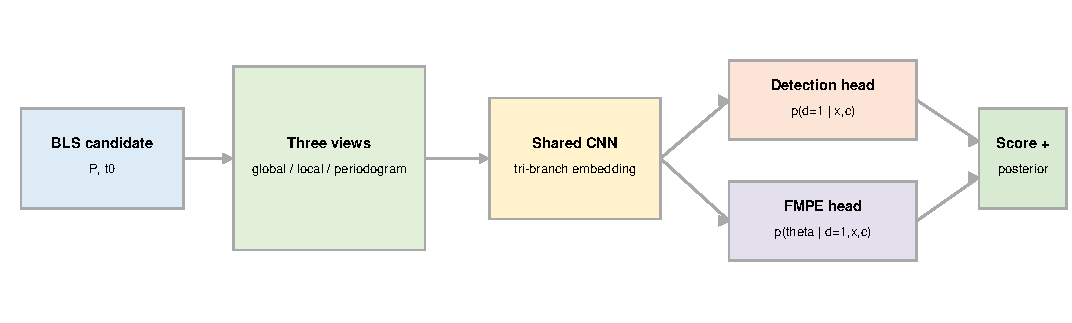
\includegraphics[width=0.98\textwidth]{figures/architecture.pdf}
 \caption{TransitFlow's candidate-conditioned task. A search algorithm proposes
 a period and epoch. Global, candidate-folded local and periodogram views feed a
 shared embedding; separate heads produce a candidate probability and an FMPE
 posterior over five transit-shape parameters. The candidate generator is part
 of any blind-search evaluation.}
 \label{fig:architecture}
\end{figure*}

\section{Forward model and neural posterior}
\label{sec:method}

\subsection{Simulator and priors}

The forward simulator produces 27-d TESS-like light curves with 18000 raw
cadences. Planet parameters are sampled from bounded priors. The period lies
between 0.5 and 13~d; $R_{\rm p}/R_\star$ is log-uniform over 0.01--0.15;
$a/R_\star$ is induced by a stellar-density prior; and grazing configurations
are included through the support of $b$. Quadratic limb darkening is sampled in
the physical $(q_1,q_2)$ parameterization of \citet{Kipping2013}. Transit curves
are exposure-integrated using a native implementation checked against
\textsc{batman} \citep{Kreidberg2015}.

The noise mixture assigns 70 per cent of examples to cached out-of-transit TESS
segments, 20 per cent to Mat\'ern-$3/2$ correlated noise plus white noise, and
10 per cent to white noise. Negative examples include eclipsing-binary-like
dips, isolated events and sinusoids. Dilution, cadence gaps and finite exposure
are simulated. A transit-preserving median filter removes slow trends. The
latest development archive contains 249 segments from 145 source-labelled
stars and is split by source target into 87/29/29 training, calibration and
evaluation groups with no target overlap. These groups support model
development, but the evaluation group has now informed model selection and
cannot serve as the final publication lockbox. Exact product provenance and a
new untouched target-level test manifest remain required.

\subsection{Representation and network}

Each curve is represented by a 2001-bin global view, a 201-bin local view folded
on $c$, and a 256-bin box-periodogram view. A tri-branch residual convolutional
network maps the views, a noise-level feature, the standardized candidate
ephemeris and a dilution feature to a 256-dimensional embedding. A binary head
returns $p(d=1\mid x,c)$. The FMPE head defines a conditional time-dependent
velocity field in prior-normal parameter space and is trained with an
optimal-transport conditional flow-matching objective,
\begin{equation}
 \mathcal{L}_{\rm FM} = \mathbb{E}
 \left\lVert v_\phi(t,\boldsymbol{z}_t\mid x,c) -
 (\boldsymbol{z}_1-\boldsymbol{z}_0)\right\rVert_2^2,
\end{equation}
where $\boldsymbol{z}_0\sim\mathcal{N}(0,I)$ and
$\boldsymbol{z}_1=\Phi^{-1}(F_{\Theta\mid P}(\boldsymbol{\theta}\mid P))$.
Here $F_{\Theta\mid P}$ is the exact prior CDF, including the support-truncated
stellar-density CDF for $a/R_\star$ conditional on period, and $\Phi$ is the
standard-normal CDF. The inverse and its Jacobian are analytic. At inference,
an ODE transports base samples to posterior samples. The evaluated model contains
approximately 4.18 million parameters and was trained for 60000 steps on one
million simulated curves.

\section{Evaluation design}
\label{sec:evaluation}

\subsection{Simulator-domain calibration}

The latest target-disjoint development diagnostic uses 500 simulated planets
and 1000 posterior samples per object. Per-parameter SBC rank histograms are
tested for uniformity with a
Bonferroni family-wise threshold of 0.05 across the five characterization
parameters. Passing such a test means that miscalibration was not detected; it
does not prove calibration. Expected coverage is measured over central credible
intervals from 5 to 95 per cent. Coverage is also stratified by $b$,
$R_{\rm p}/R_\star$, $a/R_\star$, signal-to-noise ratio and number of observed
transits.

This evaluation is useful for diagnosing the trained network but is not the
final held-out test because its failures informed the prior-normal redesign.
The final protocol will acquire and freeze a new target-level lockbox before
the model is retrained, and will keep it sealed until all model, calibration and
threshold choices are complete.

\subsection{Candidate-vetting comparison}

The original comparison constructed the neural local view from the true
positive ephemeris while requiring BLS and TLS to search the raw light curve.
That design answers different questions for the compared methods. We replace it
with a pipeline in which BLS searches each unflattened curve; its best period,
epoch and duration then define TransitFlow's preprocessing and local view. The
BLS score and TransitFlow probability are evaluated on identical examples.
Uncertainty is estimated with a stratified paired percentile bootstrap that
resamples positive and negative examples separately. The current corrected
experiment uses $n=1000$ balanced examples and 1000 bootstrap replicates.

\subsection{Real-light-curve checks}

The archived real sample consists of 30 confirmed TESS planets chosen inside
the training support and subjected to cadence, signal-to-noise and geometry
quality cuts. The published period and a data-refined epoch define the candidate.
This is a positive-only recovery study. It cannot estimate real specificity,
false-positive rate, precision or ROC-AUC.

A previous comparison used \textsc{emcee} \citep{ForemanMackey2013} on 16
objects with the ephemeris fixed. Importance weights were then used to resample
the amortized posterior before Wasserstein distances were calculated. The median
ESS fraction was 0.00181 and the minimum 0.000333, and all chains were shorter
than 50 estimated autocorrelation times. Those corrected Wasserstein values are
not scientifically interpretable. The implementation now reports raw amortized
agreement independently, records correction diagnostics without overwriting the
raw result, seeds the independent \textsc{emcee} proposal state, and gates the
reference posterior on at least 50 autocorrelation times and 400 effective
samples.

\section{Diagnostic results}
\label{sec:results}

\subsection{Pooled and conditional calibration}

The target-disjoint v4 development run has marginal SBC $p$-values 0.000,
0.019, 0.899, 0.072 and 0.000 for $R_{\rm p}/R_\star$, $a/R_\star$, $b$,
$q_1$ and $q_2$, respectively. Its pooled mean absolute expected-coverage error
is 0.015, but the familywise SBC decision fails. A bounded smoke after the
prior-normal correction, using only 6000 training cases and 3000 optimization
steps, gives p-values 0.094, 0.612, 0.117, 0.175 and 0.674 and coverage error
0.0111 on 200 separate development cases. Its calibration scales of 4.45--6.66,
large train--validation gap and detection ROC-AUC of 0.903 reveal severe
small-data overfitting. The smoke validates the corrected execution path; it is
underpowered and cannot replace the preregistered multi-seed lockbox test.

\subsection{Fair candidate-vetting pilot}

Table~\ref{tab:detection} and Fig.~\ref{fig:detection} report the corrected
candidate-level experiment. TransitFlow improves paired ROC-AUC over the BLS
score by 0.209 (95 per cent bootstrap interval 0.166--0.255) and AP by 0.178
(0.128--0.226). The absolute ROC-AUC of 0.807 is substantially below the
historical oracle-candidate value of 0.9993 on the same seeded 1000-example
simulation. BLS recovers the injected period to within 1 per cent for only
32.0 per cent of planets under the deliberately coarse 200-period search; the
median direct fractional error is near unity because harmonics are frequent.
The result shows both that candidate conditioning is useful and that candidate
generation is a dominant part of the deployed task.

\begin{table}
 \centering
 \caption{Corrected BLS-candidate comparison on 1000 simulations. Intervals are
 paired stratified bootstrap 95 per cent intervals.}
 \label{tab:detection}
 \begin{tabular}{lcc}
  \toprule
  Method & ROC-AUC & Average precision \\
  \midrule
  BLS score & 0.598 [0.561, 0.631] & 0.584 [0.551, 0.620] \\
  TransitFlow & 0.807 [0.782, 0.834] & 0.762 [0.731, 0.796] \\
  Paired gain & 0.209 [0.166, 0.255] & 0.178 [0.128, 0.226] \\
  \bottomrule
 \end{tabular}
\end{table}

\begin{figure}
 \centering
 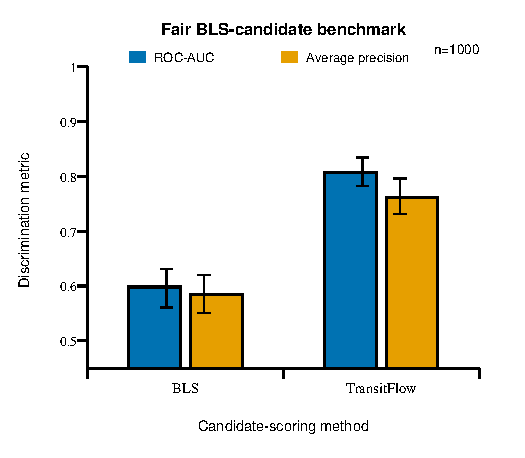
\includegraphics[width=\columnwidth]{figures/candidate_detection.pdf}
 \caption{BLS and TransitFlow discrimination when both operate in the same
 BLS-candidate pipeline. Error bars are paired-bootstrap 95 per cent intervals.
 These simulations reuse the training noise library and are therefore a pilot,
 not the final held-out benchmark.}
 \label{fig:detection}
\end{figure}

\subsection{Real recovery and posterior status}

The selected positive sample gives candidate probabilities above 0.9 for all
30 known transits. The two-sided exact 95 per cent lower confidence bound for a
30/30 binomial result is approximately 0.884, even before selection effects are
considered. The result is evidence that the network responds to high-quality
known candidates, not evidence for catalogue-level reliability.

No real-characterization agreement number is promoted to a paper result in this
draft. The archived point estimate for the prior-normalized $b$ Wasserstein
distance fluctuates across the predeclared 0.1 threshold among adjacent runs,
and the reported corrected samples have collapsed ESS. A rerun using the raw
amortized posterior and a converged, matched reference is mandatory.

\section{Discussion}
\label{sec:discussion}

The corrected experiment changes the interpretation of TransitFlow. The method
is best viewed as an amortized candidate vetter and characterization engine
downstream of a search stage. The search determines whether the local view is
coherent; training only on true positive ephemerides and random negative
ephemerides creates an avoidable train--deployment mismatch. Future training
must include BLS/TLS candidates, aliases, perturbed epochs and near-miss
candidates. The large oracle-to-deployed AUC change makes candidate robustness a
primary experiment, not an appendix.

The conditional coverage result also illustrates why pooled SBI diagnostics are
insufficient. Impact parameter is degenerate with scaled semimajor axis and limb
darkening in single-sector photometry. Stratified coverage, posterior predictive
checks and held-out real-noise groups are needed to distinguish estimator error
from simulator mismatch. Importance correction can diagnose missing support, but
an ESS of one or a few effective draws cannot repair the posterior.

The current speed measurement is likewise provisional. Amortized inference is
expected to outperform per-object MCMC after training, but a scientific speedup
must compare methods at matched accuracy and convergence on the same hardware,
include preprocessing and candidate-search cost, and state the amortization
break-even point. The archived 1659.7-fold figure does not meet all these
conditions.

\section{Blocking validation before submission}
\label{sec:blockers}

The following items are preregistered as submission gates for the next frozen
run.
\begin{enumerate}
 \item Split real-noise segments by target and sector before any injection;
 retain immutable train, validation and test manifests.
 \item Train at least three independent seeds and report seed-level outcomes,
 means, standard deviations and gate flips.
 \item Evaluate BLS, TLS and TransitFlow on the same held-out examples and
 candidate task, with paired confidence intervals, reliability diagrams and a
 modern learned vetter baseline.
 \item Freeze an untouched real sample containing confirmed planets and matched
 astrophysical/instrumental false positives, with exact MAST product identifiers.
 \item Compare raw amortized posteriors against matched MCMC or nested-sampling
 references using multiple chains, split-$\hat R<1.01$, bulk and tail ESS above
 400, and at least 50 autocorrelation times.
 \item Add FMPE--NPE, noise-regime and candidate-perturbation ablations, and
 conditional coverage with simultaneous uncertainty bands.
 \item Validate BF16 against FP32 on the same checkpoint, tensors, base draws and
 hardware with predeclared tolerances.
 \item Repeat timings only after convergence and accuracy are matched.
\end{enumerate}
The manuscript must remain marked as a pre-submission draft until every gate is
resolved or the corresponding scientific claim is removed.

\section{Conclusions}
\label{sec:conclusions}

TransitFlow implements flow-matching posterior estimation for
candidate-conditioned transit photometry and exposes a useful factorized
interface for candidate scoring and physical posterior sampling. Its pooled
simulator-domain diagnostics are promising, and a corrected candidate-level
pilot shows a paired improvement over the BLS score. The same audit also reveals
failed target-disjoint marginal calibration, strong dependence on candidate
quality, an already-inspected development evaluation, a positive-only real sample and invalid old
importance-corrected real-posterior comparisons. The scientifically honest
conclusion is therefore narrower than the original repository narrative:
TransitFlow is a promising research prototype whose MNRAS case depends on a new,
frozen and leakage-safe validation, not on the current full-run label.

\section*{Acknowledgements}

The authors acknowledge the NASA Exoplanet Archive and the Mikulski Archive for
Space Telescopes. Funding and institutional acknowledgements must be supplied by
the human authors before submission.

\section*{Author contributions}

CRediT roles and the final author list must be supplied and approved by all human
authors before submission. Artificial-intelligence systems are not authors.

\section*{Funding}

Funding information has not yet been supplied.

\section*{Conflict of interest}

The human authors must confirm the final conflict-of-interest statement before
submission. No conflict statement is inferred automatically.

\section*{AI-use disclosure}

OpenAI Codex was used as an assistive tool to inspect code and result artifacts,
identify reproducibility defects, implement and test software changes, draft
text, and generate figure code. All scientific claims, citations, analyses and
submission materials require verification and approval by the human authors.
This use must also be disclosed in the cover letter, in accordance with MNRAS
instructions.

\section*{Data availability}

The development source and diagnostic result artifacts are currently available
in the project repository. Before submission, the exact executed source,
environment, grouped data manifests, plotting tables, commands, checkpoint and
noise-library hashes, and final result bundles will be deposited in an immutable
public archive with a DOI. TESS light curves are available from MAST and catalogue
metadata from the NASA Exoplanet Archive; the final release will provide exact
product identifiers and access dates. The present draft has no archival DOI.
The 145-star development archive supports target-disjoint development, but its
evaluation partition has informed the present redesign and is not an untouched
publication lockbox.

\bibliographystyle{mnras}
\bibliography{references}

\appendix
\section{Reproducibility fields for the frozen run}

The final machine-readable manifest will include the Git commit and patch hash,
configuration, random seeds, package lock, Python/PyTorch/CUDA/cuDNN versions,
GPU model, target--sector group manifests, MAST identifiers, simulator and model
hyperparameters, primary checkpoint hash, per-object scores/posteriors, MCMC
diagnostics and all plotting data. A gate report that omits failed diagnostics is
not sufficient provenance.

\label{lastpage}
\end{document}
